%%%%%%%%%%%%%%%%%%%%%%%%%%%%%%%%%%%%%%%%%%%%%%%%%%%%%%%%%%%%%%%%%%%%%%%%
%%%%%                                                              %%%%%
%%%%% Chapter 3: SMURF-seq                                         %%%%%
%%%%%                                                              %%%%%
%%%%%%%%%%%%%%%%%%%%%%%%%%%%%%%%%%%%%%%%%%%%%%%%%%%%%%%%%%%%%%%%%%%%%%%%
\chapter{Sampling molecules using re-ligated fragments (SMURF)-seq}
\label{ch3}


%%%%%%%%%%%%%%%%%%%%%%%%%%%%%%%%%%%%%%%%%%%%%%%%%%%%%%%%%%%%%%%%%%%%%%%%
%%%%%%%%%%%%%%%%%%%%%%%%%%%%%%%%%%%%%%%%%%%%%%%%%%%%%%%%%%%%%%%%%%%%%%%%
%%%%%%%%%%%%%%%%%%%%%%%%%%%%%%%%%%%%%%%%%%%%%%%%%%%%%%%%%%%%%%%%%%%%%%%%
\section{Naive approaches to read-counting on nanopore machines}
%% Long read approach
Copy number profiling, and read-counting in general, can be done on
nanopore sequencers with long-reads ($\sim$8kb) following the standard
sequencing procedure.
% Advantages of long read sequencing
Since nanopore machines are optimized for long-read sequencing, this
method has the advantage of using any standard library preparation
protocol that are commercially available.  Sequencing long
molecules using a nanopore keeps a pore occupied for a longer duration
once a pore is loaded, followed by an open pore waiting for a molecule to
be reload.  Further, technical nucleotides, such as sequencing adapters
and barcodes, are sequenced one (or twice) every $\sim$8k bases, and
thus, the fraction of time a nanopore spends sequencing technical
nucleotides is low.
% Disadvantages of long read sequencing
However, read-counting applications do not benefit from longer reads
beyond what is necessary for unique mapping to the reference genome. In
these applications, for any fixed number of nucleotides sequenced, more
information would be obtained if those nucleotides are organized as more
DNA molecules, rather than longer contiguous fragments
(Fig.~\ref{naive_counting}).

%% Short read sequencing
An alternate approach for read-counting is to sequence short reads
($\sim$150 bp) directly on a nanopore sequencer.
%% Advantages of short read sequencing
In general, for a given sample of DNA, a nanopore instrument will
generate more reads if the corresponding molecules are shorter.  Once a
molecule is loaded into a pore, the time spent sequencing is less for
shorter reads. In addition, for a fixed amount of DNA, shorter molecules
result in higher molar concentration when loaded onto the machine,
increasing the rate at which each pore captures molecules
\citep{muthukumar2010theory,wanunu2008dna}. Therefore, sequencing short
reads on a nanopore machine would generate more reads from a sequencing
run than sequencing long reads.
%% Disadvantages of short read sequencing
However, sequencing short reads requires ad-hoc modifications to the
library preparation protocol as these are optimized for longer
molecules.  Sequencing these shorter molecules keeps a pore occupied for
a shorter duration once a pore is loaded, followed by waiting for a pore
to be reloaded (but the reload time is usually shorter due to the higher
molar concentration). Moreover, technical nucleotides are sequenced
every $\sim$150bp, increasing the fraction of time a nanopore sequences
technical bases (Fig.~\ref{naive_counting}).

\begin{figure}[b!]
\centering
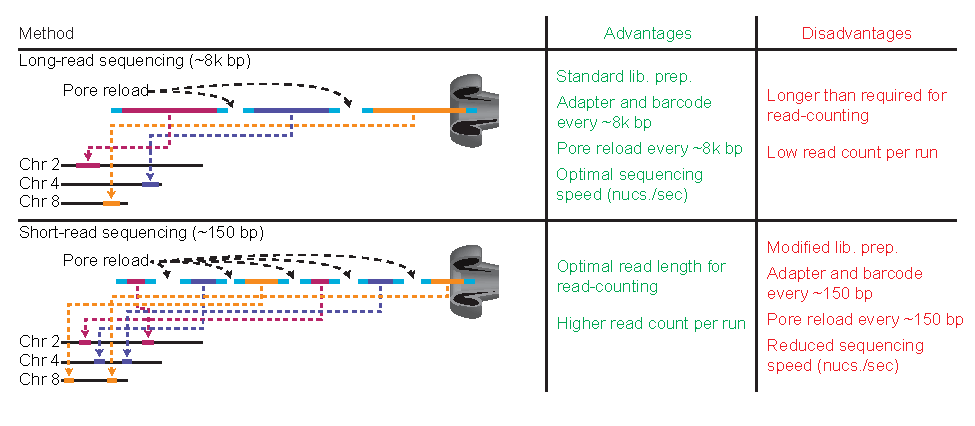
\includegraphics{naive_counting.pdf}
\caption[Naive approaches to read-counting on nanopore machines]{
  Naive approaches to read-counting on nanopore machines.
  Sequencing long-reads directly is optimized for nanopore machines but
  not for read-counting applications.
  Sequencing short-read is optimized for read-counting applications but
  not for nanopore sequencing.}
\label{naive_counting}
\end{figure}

%% SMURF-seq approach
SMURF-seq approach combines the advantages of both of these methods
and alleviates the drawbacks by using a nanopore instrument as
intended for long-read sequencing, while generating the desired short
fragments. Using the SMURF-seq approach, we generate higher read counts
per run than sequencing long or short molecules directly.


%%%%%%%%%%%%%%%%%%%%%%%%%%%%%%%%%%%%%%%%%%%%%%%%%%%%%%%%%%%%%%%%%%%%%%%%
%%%%%%%%%%%%%%%%%%%%%%%%%%%%%%%%%%%%%%%%%%%%%%%%%%%%%%%%%%%%%%%%%%%%%%%%
%%%%%%%%%%%%%%%%%%%%%%%%%%%%%%%%%%%%%%%%%%%%%%%%%%%%%%%%%%%%%%%%%%%%%%%%
\section{SMURF-seq approach to read counting}

\begin{figure}[b!]
\centering
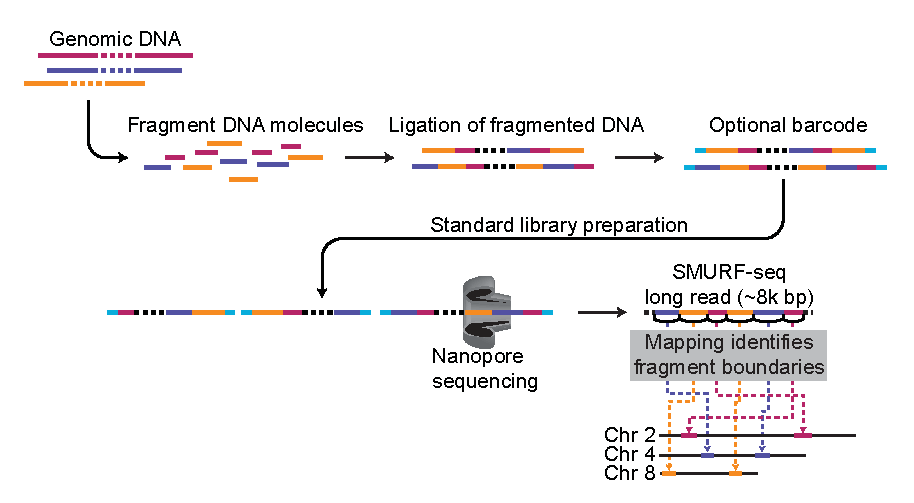
\includegraphics{smurf.pdf}
\caption[SMURF-seq approach to sequencing short fragments]{
  SMURF-seq approach to sequencing short fragments.
  SMURF-seq efficiently sequences short fragments of DNA, as required
  for read-counting applications, with a reference genome on long-read
  sequencers.
  SMURF-seq sequences short DNA molecules by generating long concatenated
  molecules from these.  SMURF-seq reads are aligned by splitting them
  into multiple fragments, each aligning to a distinct region in the
  genome.}
\label{smurf}
\end{figure}

%% SMURF-seq concept
The SMURF-seq protocol involves cleaving genomic DNA into short
fragments, with length just sufficient for an acceptable rate of
uniquely mapping fragments in the reference genome.  These fragmented
molecules are then randomly ligated back together to form artificial
long DNA molecules, as required for long-read sequencing. The long
re-ligated molecules are sequenced following the standard MinION library
preparation protocol. After (or possibly concurrent with) sequencing,
the SMURF-seq reads are mapped to the reference genome in a way that
simultaneously splits them into their constituent fragments, each
aligning to a distinct location in the genome (Fig.~\ref{smurf}).

\begin{figure}[b!]
\centering
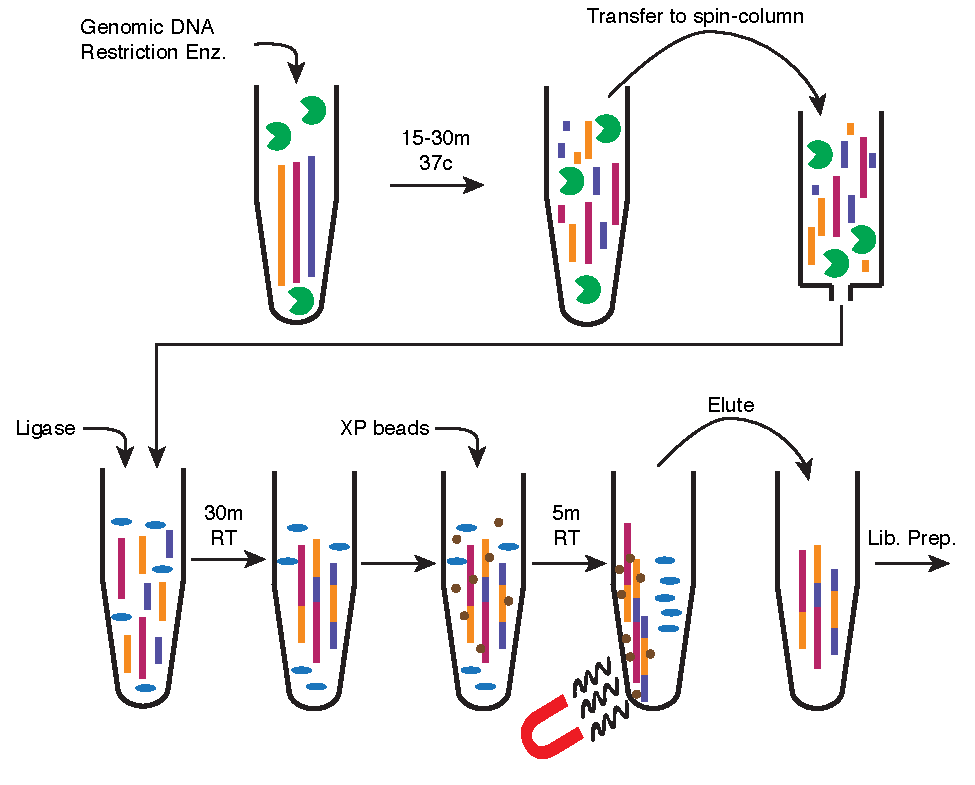
\includegraphics{ch3_fig2.pdf}
\caption[Schematic of SMURF-seq protocol]{
  Schematic of SMURF-seq protocol. SMURF-seq consists of four
  steps: restriction enzyme digestion, spin-column clean-up, re-ligation
  of fragmented DNA, and Ampure XP beads clean-up.}
\label{protocol}
\end{figure}

%% Description of SMURF-seq protocol
More specifically, genomic DNA was fragmented using restriction enzymes
and ligated with T4 DNA ligase, with clean-up steps in between.
SMURF-seq protocol is completely enzymatic and takes less than 90
minutes to complete (Fig.~\ref{protocol}).  The details of these steps
are given below:
%%
\begin{enumerate}
\item Restriction enzyme digestion: Restriction enzymes recognize
  and cleave specific DNA sequences, typically producing sticky-ended DNA
  molecules.
  %% choice of re used
  The choice of restriction enzyme used is primarily dependent on the
  size of the fragmented molecules produced. Based on the downstream
  application, this choice could also be influenced by other factors such as
  any sequence-specific biases restriction enzymes could introduce.
  %% advantages
  An advantage of using restriction enzymes to fragment DNA molecules,
  over other fragmentation techniques, is that the fragmented molecules
  have uniform ends (either sticky-ends with the same overhangs or
  blunt-ends) and are thus compatible for ligation without an end-repair
  step in between.

\item Clean-up: The reaction containing the restriction enzymes and the
  fragmented DNA molecules is cleaned to wash out the enzymes and retain
  the fragmented DNA molecules. The choice of clean-up kit used determines
  the length of the retained DNA molecules. We used a spin-column
  based clean-up that typically retains molecules that are over $\sim$70
  bp. However, other clean-up kits, such as bead-based kits, could also be
  used at this step.

\item Re-ligation: Fragmented DNA molecules with uniform ends are
  ligated at random with T4 DNA ligase enzymes.
  %% influence of time
  The most important factor in a ligation reaction is the
  concentration of compatible DNA ends \citep{dugaiczyk1975ligation}. At
  high concentrations, the chances are higher for ligation between two
  molecules than a molecule self-ligating. At low concentrations, the
  chances are higher for self-ligation.
  %%
  Thus, the main consideration during the ligation step is the
  duration of the ligation reaction, as the molar concentration of DNA
  molecules decrease with time. Too little time would lead to insufficient
  ligation, resulting in molecules of length that do not achieve optimal
  SMURF-seq efficiency. On the other extreme, too much time would result
  in circular molecules that are incompatible with the most downstream
  library preparation process. A typical ligation reaction would contain
  both short and circularized molecules, and achieving a balance between
  these determines the efficiency of SMURF-seq.
  %%
  Other factors such as the temperature and buffer contents also affect
  the ligation process.
  %% our experiments
  In our experiments, the ligation reaction was performed at a DNA
  concentration of \SI{25}{\nano\gram}$/$\SI{}{\micro\litre}
  (\SI{500}{\nano\gram} of DNA in \SI{10}{\micro\litre} nuclease-free
  water and \SI{10}{\micro\litre} DNA ligase) for \SI{30}{\minute}.

\item Bead-based clean-up: The reaction containing the ligase enzymes and
  ligated DNA molecules is cleaned to retain only the ligated molecules. We
  used a bead-based clean-up to avoid damage to long DNA
  molecules that are typical of spin-column based methods.
\end{enumerate}

\begin{figure}[b!]
\centering
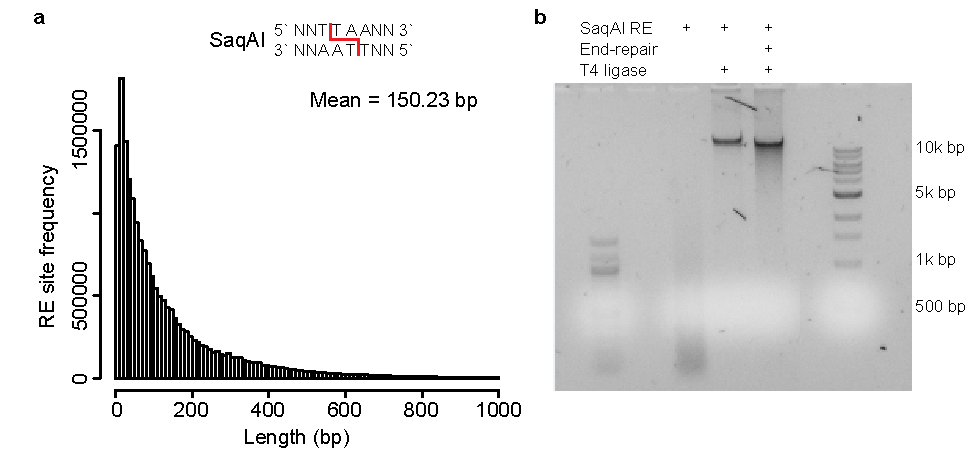
\includegraphics{ch3_fig3.pdf}
\caption[Restriction enzyme digestion and ligation of DNA molecules.]{
  Restriction enzyme digestion and ligation of DNA molecules.
  (a) Length distribution between restriction sites computed
  by measuring the distance between the recognition sites on the human
  reference genome. SaqAI recognizes the sequence TTAA and leaves a 2 bp
  overhang.
  (b) Negative gel image of fragmented and ligated DNA
  using SaqAI restriction enzyme and T4 DNA ligase.  Sticky-end and
  blunt-end ligation (by end-repair) of fragmented DNA are shown, and
  both yield ligated molecules of approximately the same length.}
\label{re_frag}
\end{figure}

%% Library construnction using standard protocols
DNA molecules that are resultant of the SMURF-seq protocol are long
molecules that are typically several kilobases, and therefore, any
standard library preparation kits that are available for nanopore
machines can be used with SMURF-seq molecules. These molecules can also
be barcoded with one (or two) barcode sequence per molecule. Thus, the
SMURF-seq approach overcomes the disadvantages of sequencing long or
short DNA molecules directly on a nanopore machine for read-counting
applications, and improves its efficiency of read-counting applications.

We also tested dsDNA fragmentase enzymes (New England Biolabs) and
acoustic shearing (Covaris) to fragment DNA. However, these methods
require an additional end-repair step after fragmentation and the
ligated molecules failed to reach the lengths we obtained by using
restriction fragmentation.

%% The sepecifics of our experiment
%% restriction digestion
In our applications, we used SaqAI restriction enzyme, which recognizes
the sequence TTAA and produces molecules with mean lengths of 150.2 bp
(Fig.~\ref{re_frag}a).
%% re-ligation
The fragmented DNA molecules are then ligated randomly to form longer
molecules using T4 DNA ligase enzyme (Fig.~\ref{re_frag}b).
%
In our experiments, the resulting long DNA molecules were prepared for
sequencing using the Oxford Nanopore Technologies 1D DNA by ligation kit
(SQK-LSK108) or the rapid sequencing kit (SQK-RAD003) following the
standard manufacturers protocol. We also multiplexed samples using the
1D native barcoding genomic DNA kit (EXP-NBD103) followed by library
preparation using the 1D DNA by ligation kit. The sequencing was
performed on a MinION instrument.
%
The detailed SMURF-seq protocol is given in Appendix~\ref{appendA}.


%%%%%%%%%%%%%%%%%%%%%%%%%%%%%%%%%%%%%%%%%%%%%%%%%%%%%%%%%%%%%%%%%%%%%%%%
%%%%%%%%%%%%%%%%%%%%%%%%%%%%%%%%%%%%%%%%%%%%%%%%%%%%%%%%%%%%%%%%%%%%%%%%
%%%%%%%%%%%%%%%%%%%%%%%%%%%%%%%%%%%%%%%%%%%%%%%%%%%%%%%%%%%%%%%%%%%%%%%%
\section{Mapping SMURF-seq reads}
The reads sequenced using SMURF-seq can be mapped to a reference genome
by first identifying short matches within the reads, corresponding to
parts of the individual fragments, and then extending those to locate
fragment boundaries.
%
As currently implemented, SMURF-seq fragments are longer than
$\sim$150bp, and mapping these reads is handled nicely using the
seed-and-extend paradigm implemented in many existing long-read mapping
tools.
%
Although none of these tools were designed to align SMURF-seq reads,
several long-read aligners such as BWA-MEM \citep{li2013aligning},
Minimap2 \citep{li2018minimap2}, and LAST \citep{kielbasa2011adaptive}
include steps designed for split-read alignment, which can be leveraged
for aligning SMURF-seq reads.

Aligning SMURF-seq reads with long-read mapping tools typically involve
variations of the following steps:
%% Steps involved in mapping SMURF-seq reads
\begin{itemize}
\item Identifying seeds: Mapping tools have a step of identifying seeds,
  which are short exactly matching parts of the read with parts of the
  reference genome. Choices in how seeds are defined and used are often
  made for mapping speed. The total size of SMURF-seq data sets is
  currently (relatively) small, so speed is not our primary concern. We
  favor the most sensitive seed strategy, but depending on implementation
  too many seed hits could lead to ambiguity later in the mapping process.
\item Chaining seeds: The identified seeds that are close to one another
  on the read and the reference, and have the same orientations
  could be merged. These are further extended into proto alignments, and
  filtered to avoid aligning potentially false-positive seed hits.
\item Aligning within the chains: In this stage a Smith-Waterman
  alignment is performed, typically allowing users to specify a mismatch
  penalty along with penalties for both gap-open and gap-extend.
\item Selecting best alignments: When high-scoring alignments overlap
  within a read, one of them (or both) could be trimmed or one is selected
  and the other discarded. The choices made here could lead to discarding
  entire fragments.
\end{itemize}

%% parameter options
Mapping tools have several parameter options, in general, these are
related to: (1) the seeding and chaining algorithm used by the
individual tool.  (2) The Smith-Waterman alignment scores, i.e. the
match score, and the mismatch and indel penalty. The seeding and
chaining parameters control the number of proto alignments that are
further refined by aligning parts of the read to the reference genome
using the specified alignment scores.

%% Importance of picking the optimal SW score
The Smith-Waterman alignment score used to align fragments to the
reference genome is crucial for determining the optimal fragment length.
On one extreme, a match score of 1 with a mismatch and indel penalty of
0 will result in one identified fragment covering the entire read and
mapping perfectly, but will always map ambiguously. On the other
extreme, a match score of 1 with a mismatch and indel penalty of
$-\infty$ will result in any mismatch or indel on the read to be
considered as a fragment boundary. Therefore, it is crucial to determine
the optimal alignment score for mapping a SMURF-seq read.

We evaluated mapping tools on simulated SMURF-seq data generated by
concatenating random fragments from real Oxford Nanopore reads. This
emulates idealized SMURF-seq reads. Within the simulated reads, the
boundaries of each fragment are known \textit{a priori}, as are their
mapping locations when in the context of their original long reads. We
used this information to evaluate mapping tools in terms of (1) how well
they identify fragments purely for the purpose of counting molecules,
which is the primary information used in CNA analysis, and (2) how well
they identify individual mapping bases within reads. After mapping these
reads, we calculated precision and recall for identifying both the
correct fragment locations, and the individual mapping bases within the
fragments (i.e. the correct fragment boundaries). Using this simulation
setup, we determined the optimal Smith-Waterman alignment score for
mapping SMURF-seq reads (detailed procedure is given in
Appendix~\ref{appendB}).

Based on these results BWA-MEM outperformed other tools, and thus, we
used BWA-MEM to align SMURF-seq reads.
%
Briefly, BWA-MEM uses short seed hits originating from different parts
of the long reads (and therefore, in our application, different
fragments within those long reads), to form clusters of seed hits in the
reference genome. Nearby clusters are joined, and then extended,
eventually resulting in (for most fragments) one alignment per fragment.
%
In our analysis, we employed BWA-MEM without any modifications to
optimize identification of fragment boundaries.  According to our
simulations, this mode of operation may not perfectly identify fragment
boundaries, but performs well in identifying mapping locations of the
individual fragments, which is the information passed to subsequent
steps in our analysis.


%%%%%%%%%%%%%%%%%%%%%%%%%%%%%%%%%%%%%%%%%%%%%%%%%%%%%%%%%%%%%%%%%%%%%%%%
%%%%%%%%%%%%%%%%%%%%%%%%%%%%%%%%%%%%%%%%%%%%%%%%%%%%%%%%%%%%%%%%%%%%%%%%
%%%%%%%%%%%%%%%%%%%%%%%%%%%%%%%%%%%%%%%%%%%%%%%%%%%%%%%%%%%%%%%%%%%%%%%%
\section{Generating higher fragment counts with SMURF-seq}
%% Long read sequencing
A typical Oxford MinION sequencing run generates approximately 500k
reads (length $\sim$8 kb) \citep{jain2018nanopore,tyson2018minion} using
the standard library preparation and sequencing protocols. Several
studies have used these long reads for copy number profiling
\citep{euskirchen2017same,magi2019nano}.

%% Short read sequencing
We tested the ability of the Oxford MinION instrument to sequence short
DNA molecules by sequencing restriction enzyme (SaqAI) digested normal
diploid genome.  The sequencing run produced 2.58 million reads with a
mean read length of 630.93 bp.
%% SMURF-seq
Using the same instrument, with SMURF-seq, we report here an average of
6.2 million mapped fragments per run, which is substantially more
fragments than directly sequencing long or short reads directly.
Further, the SMURF-seq approach generated fragments at a substantially
faster rate than sequencing short molecules directly
(Fig.~\ref{frag_time}).

\begin{figure}[t!]
\centering
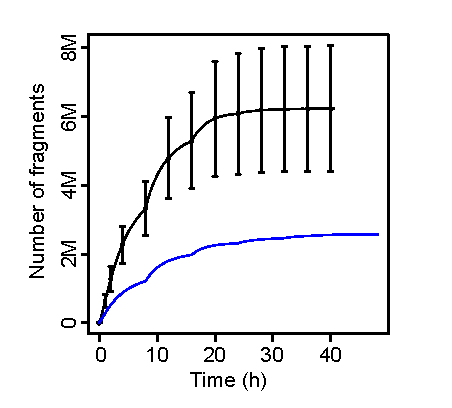
\includegraphics{frag_time.pdf}
\caption[SMURF-seq generates fragments at a faster rate than
  sequencing short molecules directly.]{
  SMURF-seq generates fragments at a faster rate than sequencing
  short molecules directly. Number of fragments obtained from reads
  plotted as a function of  sequencing time. For SMURF-seq, the average
  number of fragments from runs using the 1D sequencing by ligation kits
  are plotted (error bars indicate one standard deviation). For short-read
  sequencing run, each read is considered as one fragment.}
\label{frag_time}
\end{figure}

%% Why does SMURF-seq perform better?
% pore reload time
The most important factor in the performance of SMURF-seq over
sequencing short molecules directly is that sequencing concatenated
fragments effectively eliminates the pore reload time for all but the
first fragment in each read. However, there are a variety of additional
factors that favor further optimization of the approach employed by
SMURF-seq.
% sequences fewer technical bases
First, reduction of resources spent on technical nucleotides: SMURF-seq
uses a single barcode and sequencing adapter per read consisting of
multiple fragments; sequencing short reads uses one barcode and adapter
per fragment, adding approximately 50 bases to each fragment. This
increases the time to sequence each short read. In sequencing short
reads, as the reads get shorter the time consumed by these technical
bases increases. In SMURF-seq, sequencing either shorter fragments in
fixed length reads, or longer reads containing fragments of fixed
average length, both reduce the time consumed sequencing these technical
bases.
%
In the limit, assuming 100bp DNA fragments, sequencing those fragments
as short-reads corresponds to 33\% technical nucleotides; for SMURF-seq,
the portion of technical nucleotides remains low.
% Nanopores sequence at full speed
Second, more nucleotides sequenced at full speed: We observed that the
speed of sequencing was lower when sequencing short molecules. For
example, the average sequencing speed was 315.54 bases per second for
sequencing the diploid genome without SMURF-seq, and 400.29 bases per
second when sequencing using SMURF-seq on the MinION sequencer.
% Compatible with all library prep kits
Third, leveraging optimizations to long-read protocols: The rapidly
evolving nanopore library construction kits are continually optimized
for long-read sequencing, and would likely require significant ad-hoc
modifications to optimize sequencing of short molecules of length
optimal for read-counting applications.


%%%%%%%%%%%%%%%%%%%%%%%%%%%%%%%%%%%%%%%%%%%%%%%%%%%%%%%%%%%%%%%%%%%%%%%%
%%%%%%%%%%%%%%%%%%%%%%%%%%%%%%%%%%%%%%%%%%%%%%%%%%%%%%%%%%%%%%%%%%%%%%%%
%%%%%%%%%%%%%%%%%%%%%%%%%%%%%%%%%%%%%%%%%%%%%%%%%%%%%%%%%%%%%%%%%%%%%%%%
\section{Efficient CNA profiling using SMURF-seq}
To demonstrate the utility of SMURF-seq, we generated CNA profiles of
normal diploid and highly rearranged cancer genomes.  The mapped
fragments were grouped into variable length ``bins'' across the genome
and bin counts were used to generate CNA profiles as described in
\cite{baslan2012genome} and \cite{kendall2014computational}.

\subsection{Accurate CNA profiles using SMURF-seq}
\begin{figure}[t!]
\centering
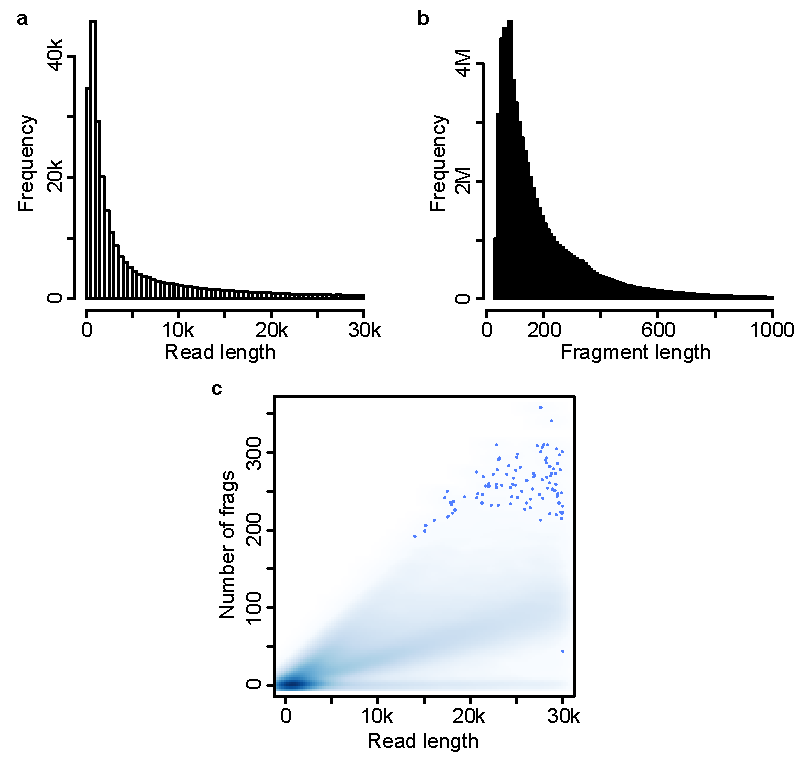
\includegraphics{read_frag_dist.pdf}
\caption[Read and fragment lengths from a SMURF-seq sequencing run.]{
  Read and fragment lengths from a SMURF-seq sequencing run.
  (a) Sequenced read length distribution.
  (b) Mapped fragment length distribution.
  (c) Scatter plot of read length and the number of fragments contained
  in the read.}
\label{read_frag_dist}
\end{figure}

%% Diploid genome
We sequenced a normal diploid female genome with SMURF-seq, resulting in
270.8k reads (mean read length of 6.75 kb) in a single run. These reads
were split into 7.28 million fragments (26.87 mean fragments per read;
Fig.~\ref{read_frag_dist}).  A CNA profile for this normal diploid
genome, with the expected (approximately flat) appearance can be seen in
Fig.~\ref{cnv}a.
% Replicate
A replicate of this experiment resulted in 497.9k reads (mean read
length of 3.7 kb), which were split into 7.55 million fragments (15.16
mean fragments per read).

%% Rapid kit
The rapid sequencing kit form Oxford Nanopore Technologies offers an
extremely fast (10 minute) and simple (2 step) protocol for library
preparation. We verified that the SMURF-seq procedure behaves similarly
using the rapid sequencing kit. The 213.38k sequenced reads had a mean
read length of 3.9 kb, and were split into 2.81 million fragments.  The
copy number profile of the diploid genome was flat, as expected.

%% skbr3 genome
Next, we applied SMURF-seq to the breast cancer line SK-BR-3, generating
147.0k reads with mean length of 7.62 kb, which were split into 4.52
million fragments (30.78 mean fragments per read). We then obtained a
CNA profile using 5,000 bins, corresponding to an average bin size of
approximately 600 kb (Fig.~\ref{cnv}b).

\begin{figure}[b!]
\centering
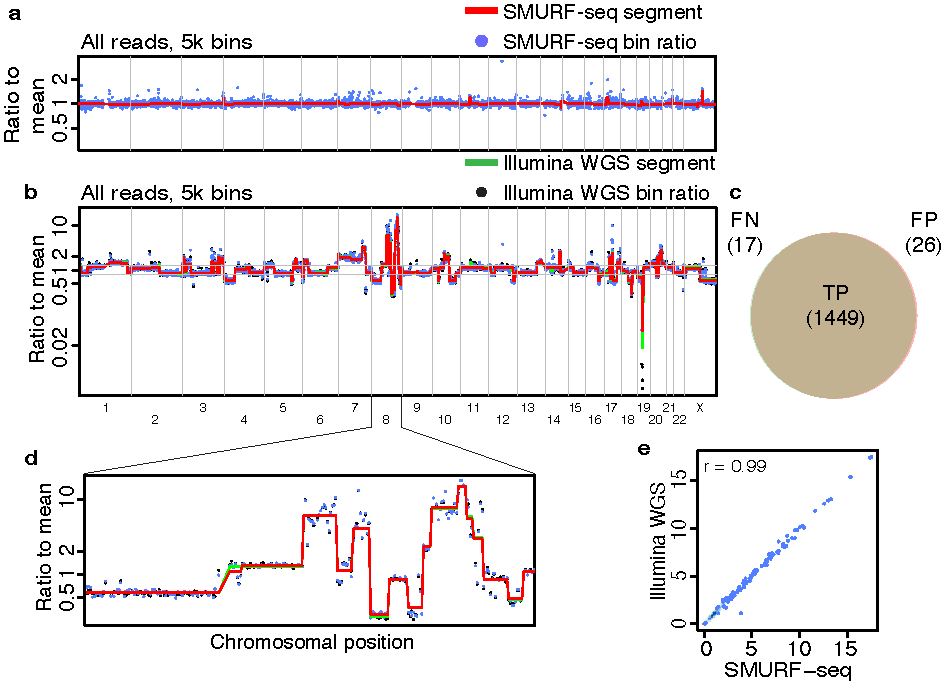
\includegraphics{ch3_fig4.pdf}
\caption[Accurate copy number profiles with SMURF-seq.]{
  Accurate copy number profiles with SMURF-seq.
  (a) CNA profile of a normal diploid genome. Each blue point is a
  bin ratio to mean and the red line is the segmented bin ratio.
  (b) Superimposed CNA profiles of SK-BR-3 genome generated using
  SMURF-seq and Illumina WGS reads.
  (c) Venn diagram illustrating the accuracy of event calls using
  SMURF-seq compared with Illumina WGS.
  (d) Zoom-in of copy number changes on chromosome 8.
  (e) Scatter plot of bin ratio of SK-BR-3 genome using
  SMURF-seq and Illumina WGS reads. Pearson correlation of the data
  is shown.}
\label{cnv}
\end{figure}

To provide a quantification of accuracy in terms of individual CNA
events we conducted whole-genome sequencing (WGS) on the same SK-BR-3
using Illumina (5.56 million reads; 130 bp, single-end).  We used this
to define a ground truth by calling CNA events for each of the
pre-defined bins (both amplifications and deletions) based on the
segmented signal with a cutoff of 1.25/0.8 (Fig.~\ref{cnv}b)
\citep{dago2014rapid,berry2017potential}. This resulted in 1,466 events
(886 amplifications, 580 deletions) from 4,953 bins. We then called
events using the identical procedure with SMURF-seq data from the same
SK-BR-3 sample. The precision and recall for SMURF-seq relative to the
Illumina calls were 0.982 and 0.988, respectively (Fig.~\ref{cnv}c).
Fig.~\ref{cnv}d shows a zoom-in of a region with extreme copy number
alterations. The bin ratios for the Illumina WGS and the SMURF-seq
profiles are highly correlated (Pearson $r$ = 0.99; Fig.~\ref{cnv}e).
% replicate
A replicate of this experiment resulted in 132.64k reads (mean read
length of 7.3 kb), which were split into 4.02 million fragments (30.31
mean fragments per read).

\begin{figure}[t!]
\centering
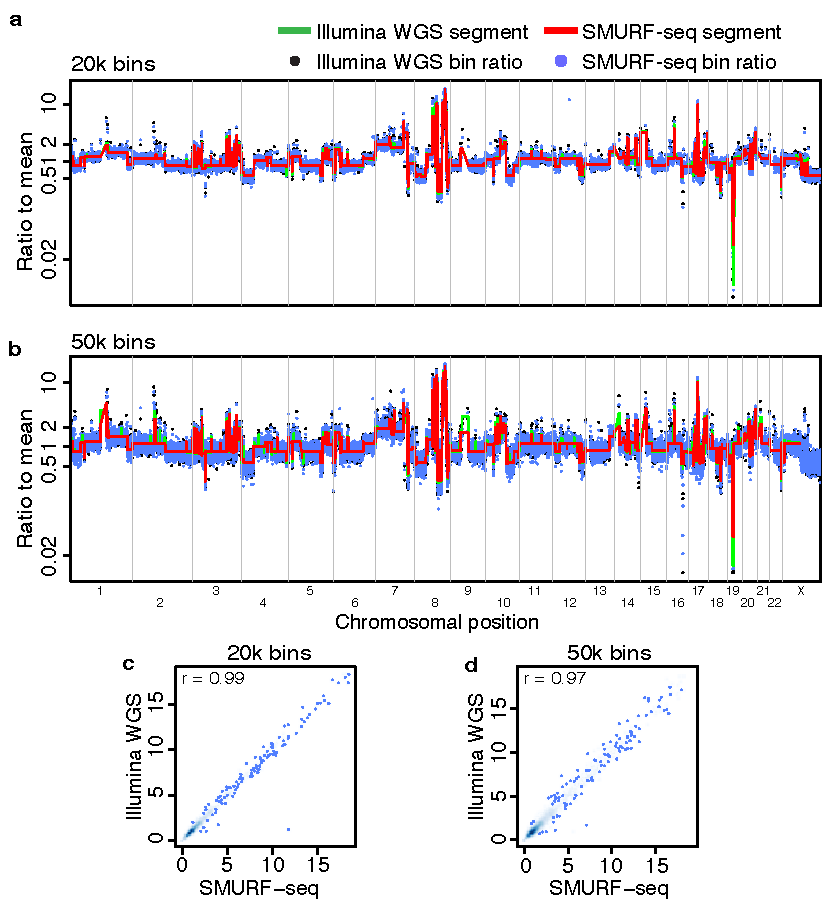
\includegraphics{skbr3_hi_res.pdf}
\caption[High-resolution CNA profile with SMURF-seq]{
  High-resolution CNA profile generated using SMURF-seq is highly concordant
  with the profile generated with Illumina WGS.
  (a, b) Superimposed CNA profiles of SK-BR-3 genome generated using SMURF-seq
  and Illumina WGS at 20,000 and 50,000 bin resolutions.
  (c, d) Scatter plot of bin ratios of SK-BR-3 genome using
  SMURF-seq and Illumina WGS reads at 20,000 and 50,000 bin resolutions.
  Pearson correlation of the data is shown.}
  \label{skbr3_hi_res}
\end{figure}

%% Hige resolution profiles
We also generated higher-resolution CNA profiles with 20,000 and 50,000
bins, corresponding to an average of approximately 150 kb and 60 kb in
length, respectively (Fig.~\ref{skbr3_hi_res}a, b). The profiles obtained
at these resolutions have a high correlation with the profiles obtained
using Illumina WGS (Pearson $r>$ 0.97; Fig.~\ref{skbr3_hi_res}c, d).

\subsection{Concordant profiles from fewer countable fragments}
\begin{figure}[t!]
\centering
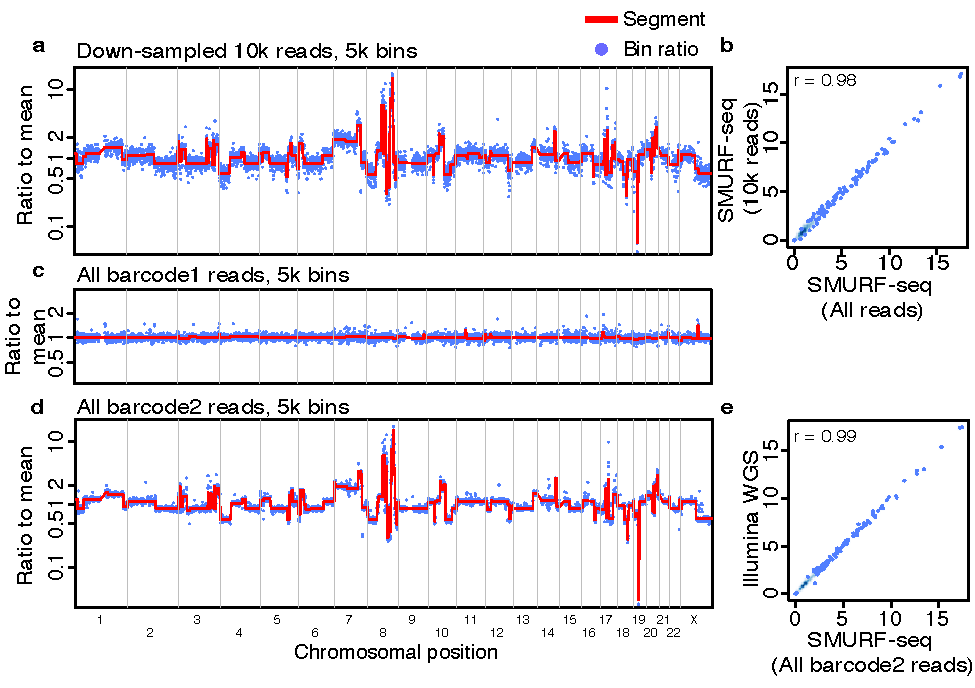
\includegraphics{ch3_fig5.pdf}
\caption[Multiple SMURF-seq CNA profiles by multiplexing in a single run]{
  Multiple SMURF-seq CNA profiles by multiplexing in a single run.
  (a) CNA profile of SK-BR-3 genome with down-sampled 10k SMURF-seq reads.
  (b) Scatter plot of normalized bin counts of the original SMURF-seq
  data and data down-sampled to 10k SMURF-seq reads. Pearson
  correlation of the data is shown.
  (c) CNA profile of barcode01 (Normal diploid genome) reads.
  (d) CNA profile of barcode02 (SK-BR-3 cancer genome) reads.
  (e) Scatter plot of bin ratios of SK-BR-3 genome using
  multiplexed SMURF-seq and Illumina WGS reads.}
\label{cnv_mux}
\end{figure}

Several cancer-related studies have employed CNA profiling based on
low-coverage WGS \citep{macintyre2018copy,kader2016copy}.  It has
previously been demonstrated that 250k reads are sufficient for accurate
genome-wide CNA profiling of single cells \citep{baslan2015optimizing}.
At the same time, the CNA profiles from a population of cells has been
shown to have a high correlation with single-cell profiles
\citep{navin2011tumour,baslan2015optimizing}. We reasoned that using
250k fragments for CNA profiling using a population of cells would give
useful profiles if they remained sufficiently accurate.  By
down-sampling our SMURF-seq data, we verified that 10k reads,
approximately 250k fragments, result in highly-correlated CNA profiles
(Pearson $r$ = 0.98; Fig.~\ref{cnv_mux}a, b).

Given the total capacity of the MinION instrument, this indicates that
multiple samples can effectively be barcoded and multiplexed in a single
sequencing run.
%%
To verify this, we sequenced two DNA samples (normal diploid female and
SK-BR-3) in a single run.  These samples were processed with SMURF-seq
protocol and then barcoded following the standard library construction.
After demultiplexing and mapping the reads, the diploid genome had a CNA
profile as expected (Fig.~\ref{cnv_mux}c) and the SK-BR-3 CNA profile
was nearly identical to the profile obtained using Illumina WGS (Pearson
$r$ = 0.99; Fig.~\ref{cnv_mux}d, e). All the sequencing runs and the
availability of sequence data are summarized in Appendix~\ref{appendC}.

\begin{figure}[t!]
\centering
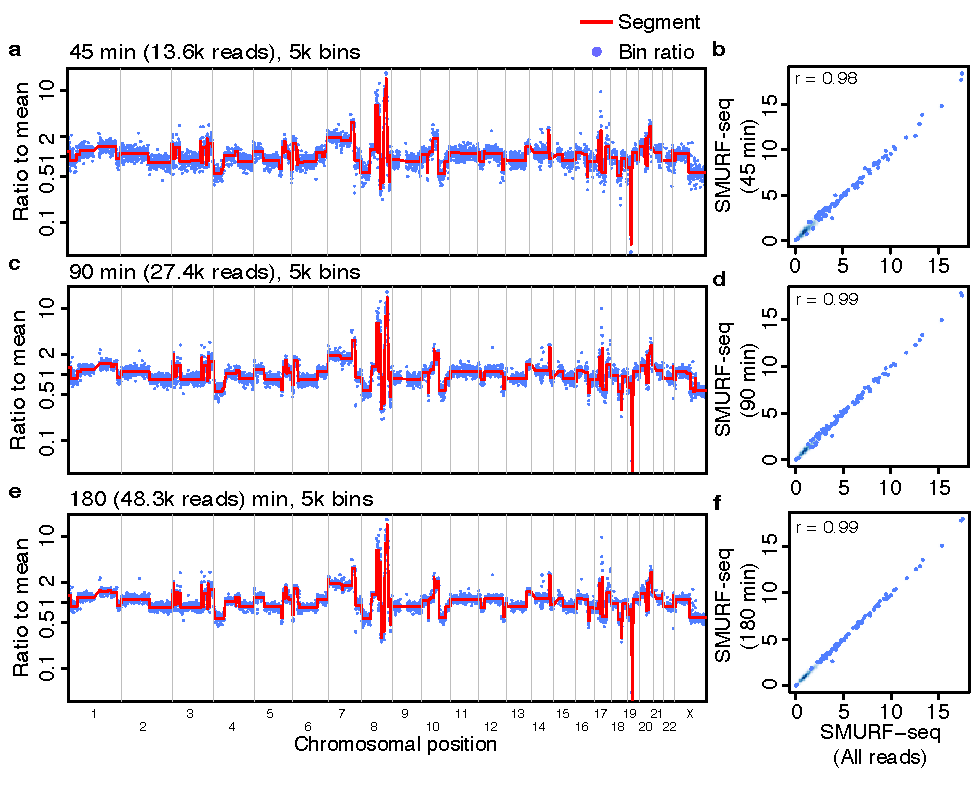
\includegraphics{cnv_time.pdf}
\caption[CNA profile with reads obtained in first few minutes of
  sequencing]{
  CNA profile with reads obtained in first few minutes of sequencing.
  (a, c, e) CNA profile  with reads obtained in the first 45, 90,
  and 180 minutes of sequencing.
  (b, d, f) Scatter plot of bin ratios of the original
  SMURF-seq data and data obtained in first 45, 90, and 180
  minutes of sequencing. Pearson correlation of the data is shown.}
  \label{cnv_time}
\end{figure}

%% Terminating sequencing early
Further, we verified that the CNA profile with reads generated in the
first 45, 90, and 180 minutes of starting a sequencing run had a high
correlation to the profile with reads from the complete run (Pearson
$r>$ 0.98; Fig.~\ref{cnv_time}).

In summary, our results demonstrate that SMURF-seq can generate more
information for CNA analysis in a single run of the Oxford MinION
sequencer, compared with either sequencing long reads in the usual way
or direct short-read sequencing on the same instrument.  This increased
information is in the form of increased numbers of distinct DNA
fragments sequenced, and can be leveraged in multiple ways. Applying
SMURF-seq on a single sample for a full run corresponds to higher counts
for downstream analysis. In CNA analysis, increased counts either add
confidence for a fixed resolution, or can allow higher resolution
analysis (i.e. smaller bins) at the same level of confidence.
Alternatively, the increased information throughput can effectively
reduce the time required to produce the same number of counts for CNA
analysis by terminating the sequencing earlier. Finally, the increased
information yield can be directed towards reducing the cost of
generating CNA profiles by allowing a greater degree of multiplexing.
For CNA analysis at resolutions permitted by 250k mapped fragments, our
results show SMURF-seq allows roughly 20 and up to 30 samples in a
single run, compared with 10 per run directly using short-read
sequencing.

%%%%%%%%%%%%%%%%%%%%%%%%%%%%%%%%%%%%%%%%%%%%%%%%%%%%%%%%%%%%%%%%%%%%%%%%
%%%%%%%%%%%%%%%%%%%%%%%%%%%%%%%%%%%%%%%%%%%%%%%%%%%%%%%%%%%%%%%%%%%%%%%%
%%%%%%%%%%%%%%%%%%%%%%%%%%%%%%%%%%%%%%%%%%%%%%%%%%%%%%%%%%%%%%%%%%%%%%%%
\section{Future of SMURF-seq}
\label{future_smurf}

\subsection*{SMURF-seq with shorter fragments}
For CNA profiling with SMURF-seq, we used restriction enzyme SaqAI which
fragments the human genome generating molecules with a mean length of
150 bp. For CNA profiling and other read-counting applications, the
length of the fragmented molecules needs to be just long enough to
ensure unique mappability to a sufficient fraction of the genome. Thus,
reducing the fragment lengths could increase the number of fragments in
a SMURF-seq read, and would increase the number of read-counts obtained
per sequencing run.

% RE digestion with multiple enzymes
The length of the fragmented DNA molecules can be reduced by digestion
with a combination of restriction enzymes, as these would recognize more
sites on the genome. Depending on the choice of enzymes used, the
fragmented molecules could have blunts-ends, sticky-ends that are not
compatible with one another for ligation, or a combination of blunt and
sticky-ends.
%
These fragmented DNA could be end-repaired to have blunt ends on all
molecules prior to ligation. However, this step adds an end-repair and a
clean-up step (after end-repair) to the SMURF-seq protocol.
%
Another option is to directly ligate the fragmented molecules even
though they do not have compatible ends. As an example, after digestion
with two restriction enzymes that generate different ends, the
fragmented molecules can be of three types: The fragmented molecule
could have both ends from the first enzyme, both ends from the second
enzyme, or one end from each of the enzymes. Ligating these molecules
directly (i.e. without end-repair) would concatenate the two types of
molecules that have the same ends within each type; the type of
molecules that have two different ends would act as bridges between the
molecules that have the same ends. Although, this protocol would have
fewer steps, the efficiency of ligation could be reduced and would need
to be evaluated.

% implication on read-counting
The use of restriction enzymes or a combination of enzymes for
fragmentation could lead to a bias in read counts for the downstream
application. For example, in terms of copy number profiling, the number
of restriction sites in a bin could vary, causing variation in bin
counts that does not reflect the sequenced sample. The effect of the
biases needs to assessed based on the enzymes used and the downstream
application.

% other techniques for fragmentation

\subsection*{Sequencing fragmented molecules with SMURF-seq}
% pre-fragmented DNA molecules
Some read-counting applications, such as Ribo-seq
\citep{ingolia2009genome}, involve extensive steps to produce the
molecules of interest. The resultant DNA molecules from these
protocols could already be fragmented to length optimal for SMURF-seq.
Other applications such are targeted-capture methods and whole-exome
sequencing protocols typically produce molecules that are $\sim$150-200
bp. Further, cell-free DNA molecules obtained from blood samples are of
length $\sim$150 bp, and are increasingly used in low-coverage copy
number profiling \citep{underhill2016fragment,
adalsteinsson2017scalable}.

\begin{figure}[t!]
\centering
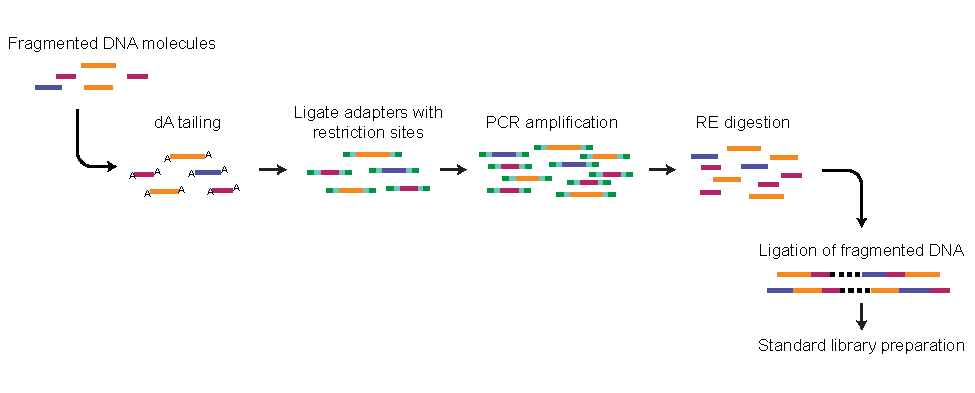
\includegraphics{fraged_smurf.pdf}
\caption[SMURF-seq protocol to sequence pre-fragmented DNA molecules]{
  SMURF-seq protocol to sequence DNA molecules that are
  already fragmented. The light green bands
  on the adapters represent restriction sites. These molecules are
  amplified with an adapter containing a restriction site, followed by
  restriction digestion, and re-ligation for sequencing on long-read
  machines.}
\label{fraged_smurf}
\end{figure}

Sequencing these molecules using SMURF-seq would require that these
molecules have compatible ends for ligation, and the quantity of DNA is
sufficient for nanopore sequencing.
% protocol
To meet these requirements, DNA molecules from these protocols could be
PCR amplified by first dA-tailing and ligating adapters to bind the PCR
primers. If these adapters are designed to have an appropriate
restriction site in them, after amplification they could be removed with
restriction digestion, leaving behind DNA molecules with sticky-ends as
required for SMURF-seq (Fig~\ref{fraged_smurf}).

%% additional sequence
Designing PCR adapters with restriction sites  also provides an
opportunity to insert an additional sequence in an adapter prior to
restriction site. This sequence could be modified depending on the
downstream application. For example, it could be a barcode sequence or a
unique molecular identifier sequence.

However, SMURF-seq is still limited by the number of fragments produced
from a run on the sequencing instrument.  We believe that the evolution
of SMURF-seq and the improvements to the underlying sequencing
technology would expand the utility of SMURF-seq, enabling applications
on nanopore instruments that are currently only possible with short-read
high-throughput machines.
